\documentclass{beamer}
\usepackage[latin1]{inputenc}
%\usetheme[noshadow,nonav,nologo]{NYU}
\usetheme[numbers]{NYU}
\usepackage{amsmath}
\usepackage{amsfonts}
\usepackage{amssymb}
\usepackage{color, colortbl}

\makeatletter
\newcommand{\thickhline}{%
    \noalign {\ifnum 0=`}\fi \hrule height 2pt
    \futurelet \reserved@a \@xhline}

\title{Saturating Auto-Encoder}
\date{December 12, 2012} 
\author{Ross Goroshin}

\begin{document}


\begin{frame} 
\frametitle{Contractive Auto-Encoder}
\begin{itemize}
\item{A technique of obtaining "interesting" representations is to regularize the latent representation}
\item{Contrary to more traditional regularization directly on weights, these correspond to "generic prior hypotheses"}
\item{$L_{CAE} = \sum_{x \in D_n} \|x-x_r\|_2 ^2 + \lambda \sum_{ij} \left(\frac{\partial h_j(x)}{\partial x_i} \right)^2$ }
\end{itemize} 
\begin{center}
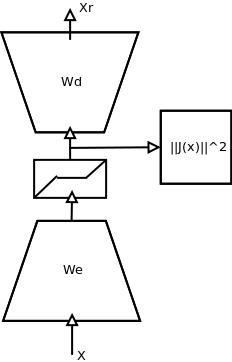
\includegraphics[scale = 0.4]{CAE.png} 
\end{center} 
\end{frame} 

\begin{frame}
\frametitle{Contractive AE} 
\begin{itemize}
\item{$\left(\frac{\partial h_j(x)}{\partial x_i}\right)^2 = (h'_j(x))^2 W_{e_{ij}}^2$}
\item{Important to tie or normalize weights}
\item{If there were no reconstruction objective then the penalty on the Jacobian would produce a constant representation for all inputs either by saturating or weight decay} 
\item{However nearby data-points on the manifold must be distinctly reconstructed}
\item{The contractive pressure is counteracted by the reconstruction gradient in the directions tangent to the manifold}
\item{Can be interpreted roughly as curvature regularization}
\end{itemize} 
\end{frame} 

\begin{frame}
\frametitle{Auto-Encoders}
\begin{itemize}
\item{The goal is to obtain a good representation (parameterization) of the data-manifold}
\item{The reconstruction objective ensures that points on the manifold are well reconstructed (pushes down energy or raises probability)} 
\item{Without any other constraints, it often means that points that are off the data manifold are also well reconstructed} 
\item{This is not an issue when maximizing log-likelihood}  
\begin{center}
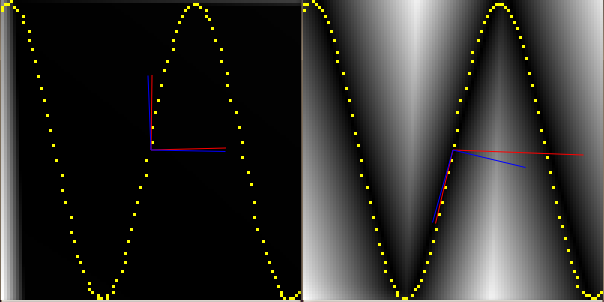
\includegraphics[scale = 0.2]{psh_and_pull.png} 
\end{center} 
\end{itemize} 
\end{frame} 

\begin{frame}
\frametitle{Saturating Auto-Encoder (SAE)} 
\begin{itemize}
\item{Inspired by the CAE, we introduce a penalty on activations outside the saturated region of the nonlinearity} 
\begin{center}
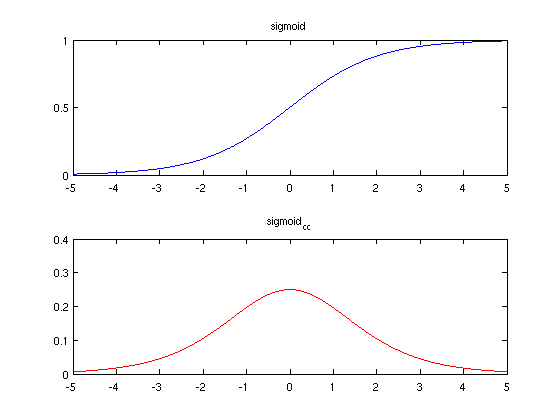
\includegraphics[scale = 0.20]{sigmoid_cc.png}
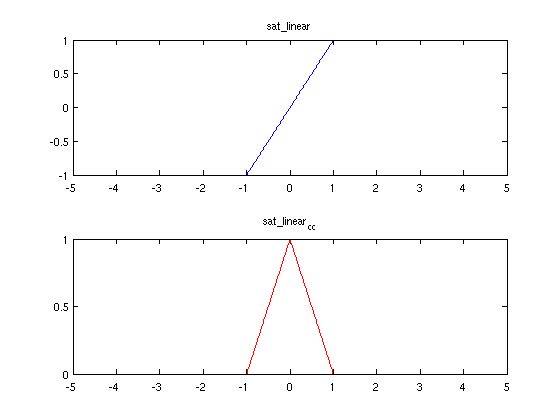
\includegraphics[scale = 0.20]{sat_linear_cc.png} 
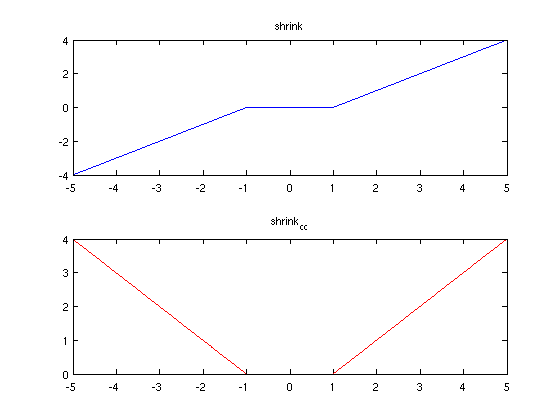
\includegraphics[scale = 0.20]{shrink_cc.png} \\
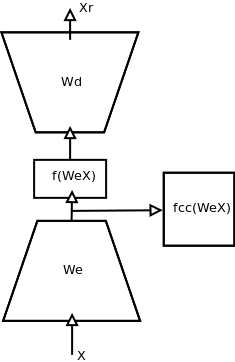
\includegraphics[scale = 0.20]{SAE.png}
\end{center} 
\end{itemize} 
\end{frame} 

\begin{frame}
\frametitle{SAE: $shrink()$ nonlinearity} 
\begin{center} 
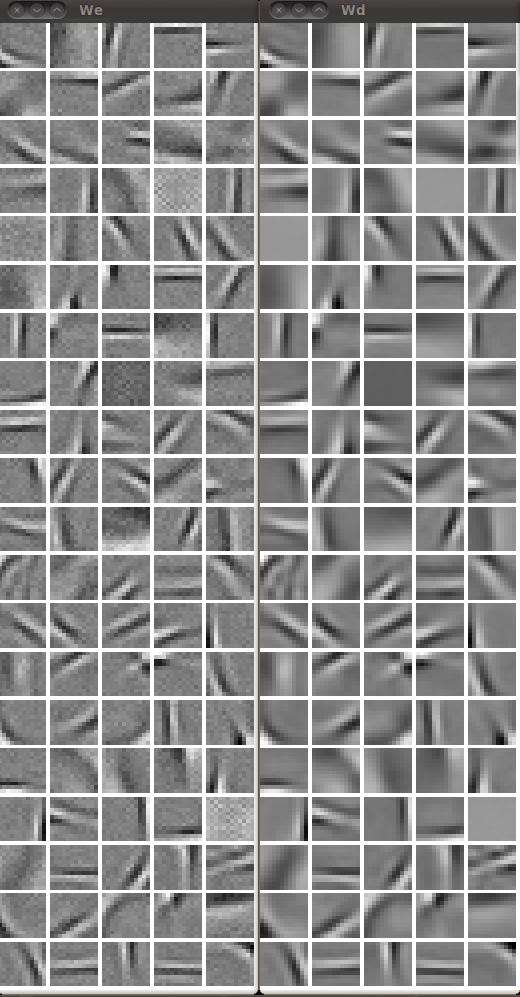
\includegraphics[scale = 0.20]{Wshrink.png}
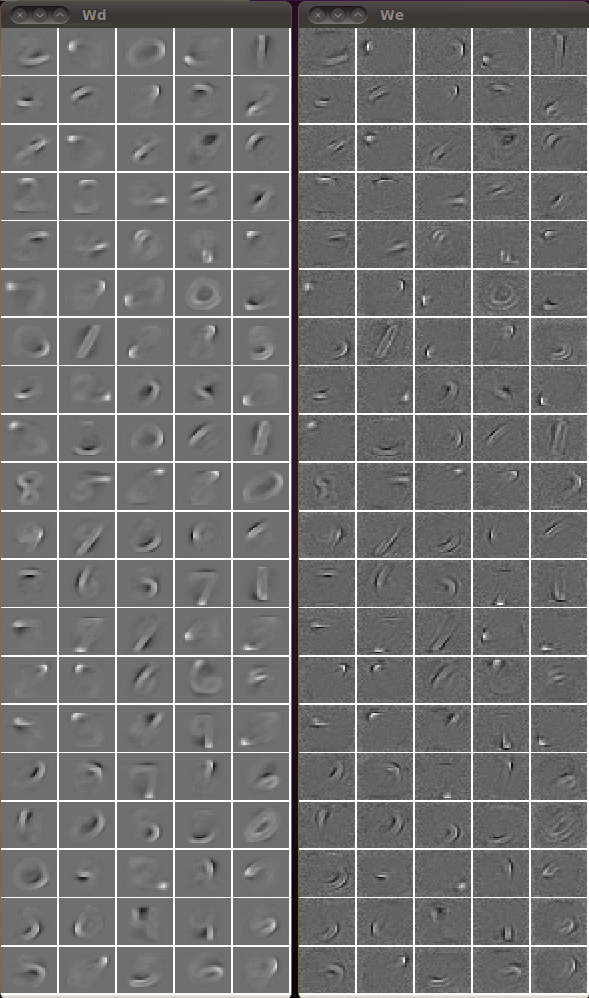
\includegraphics[scale = 0.20]{strokes.png}
\end{center} 
\end{frame} 

\begin{frame}
\frametitle{SAE: $sat\_linear()$ nonlinearity} 
\begin{center} 
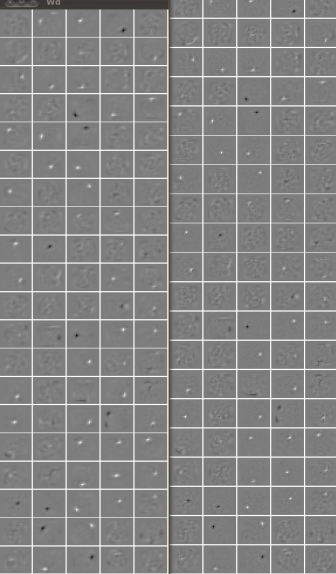
\includegraphics[scale = 0.35]{sat100.png}
\end{center} 
\end{frame} 

\begin{frame}
\frametitle{SAE: $sat\_linear()$ nonlinearity} 
\begin{center} 
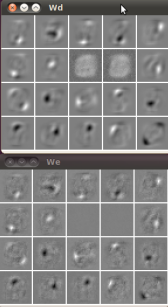
\includegraphics[scale = 0.45]{sat20.png}
\end{center} 
\end{frame} 

\begin{frame}
\frametitle{SAE: $sat\_linear()$ nonlinearity} 
\begin{center} 
Reconstruction error surface for $\eta = 0, 0.05, 0.1, 0.2$ 
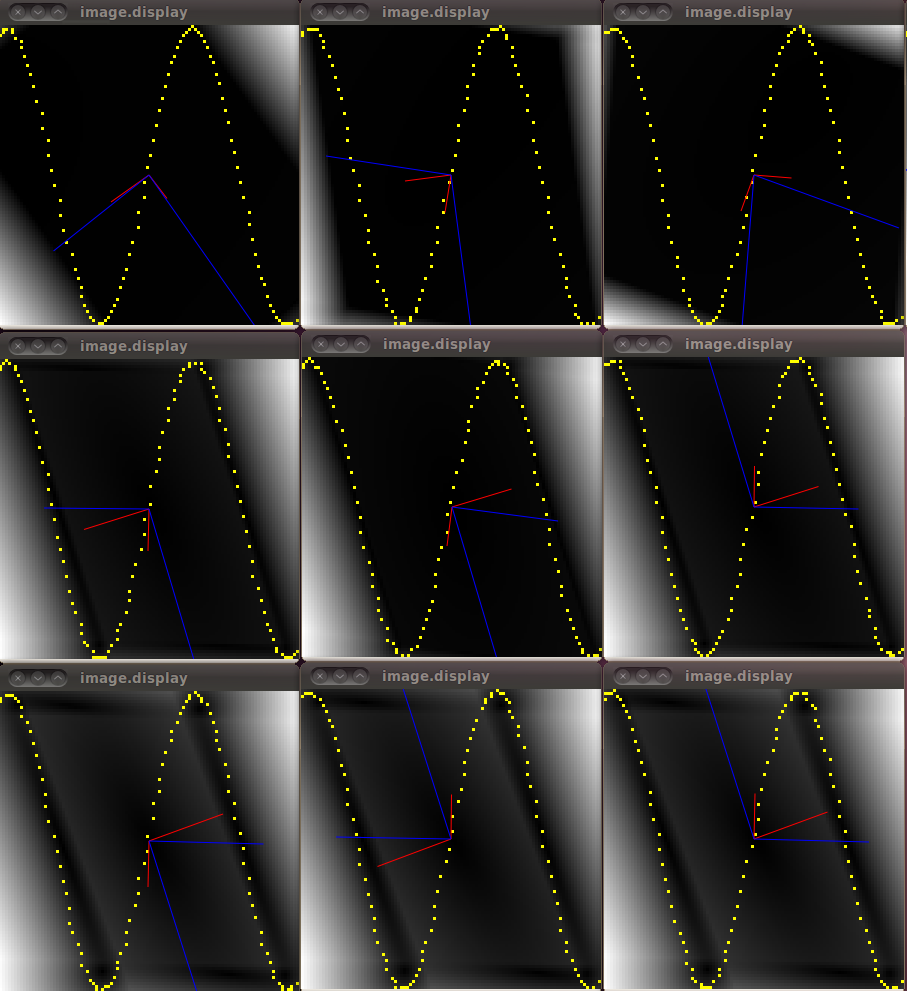
\includegraphics[scale = 0.15]{sat_linear_result0to02.png}\\
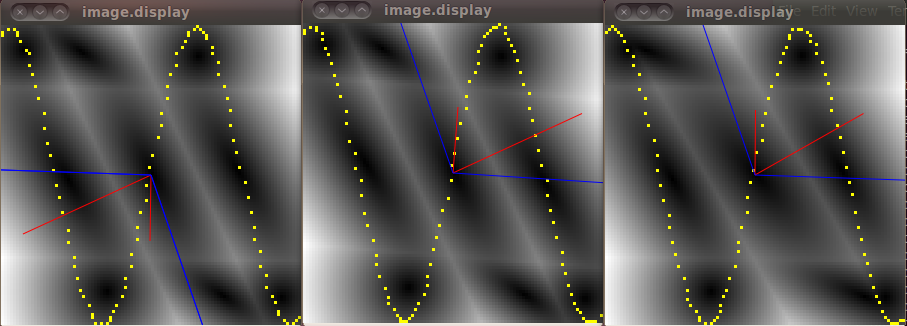
\includegraphics[scale = 0.15]{sat_linear_result03.png}
\end{center} 
\end{frame} 

\begin{frame}
\frametitle{SAE: $sat\_linear()$ nonlinearity} 
\begin{center}
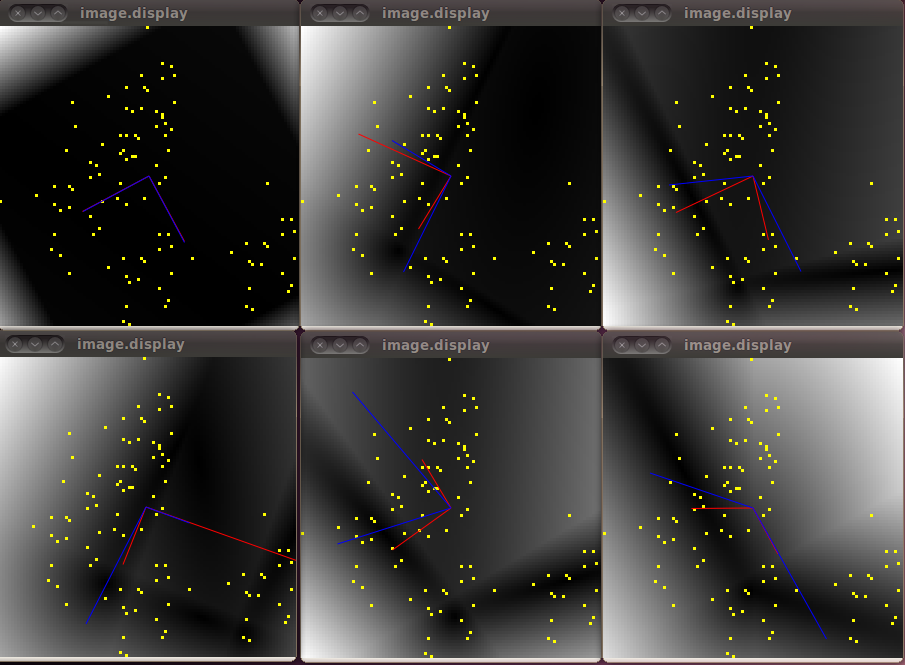
\includegraphics[scale = 0.3]{sat_linear_scatter.png}
\end{center} 
\end{frame} 

\begin{frame}
\frametitle{SAE: $sat\_linear()$ nonlinearity} 
\begin{center}
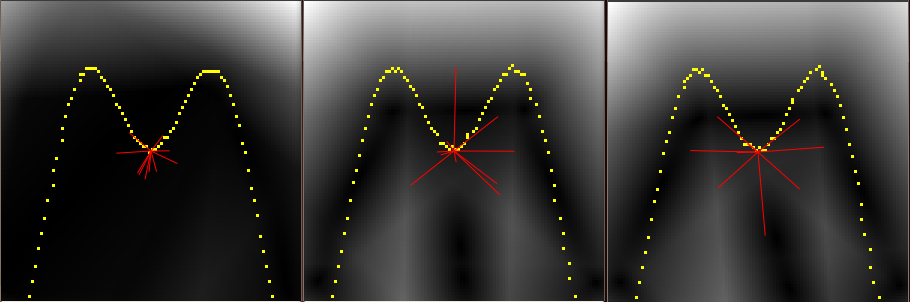
\includegraphics[scale = 0.3]{sat_linear_M.png}
\end{center} 
\end{frame} 

\begin{frame}
\frametitle{SAE: $shrink_+()$ nonlinearity} 
\begin{center}
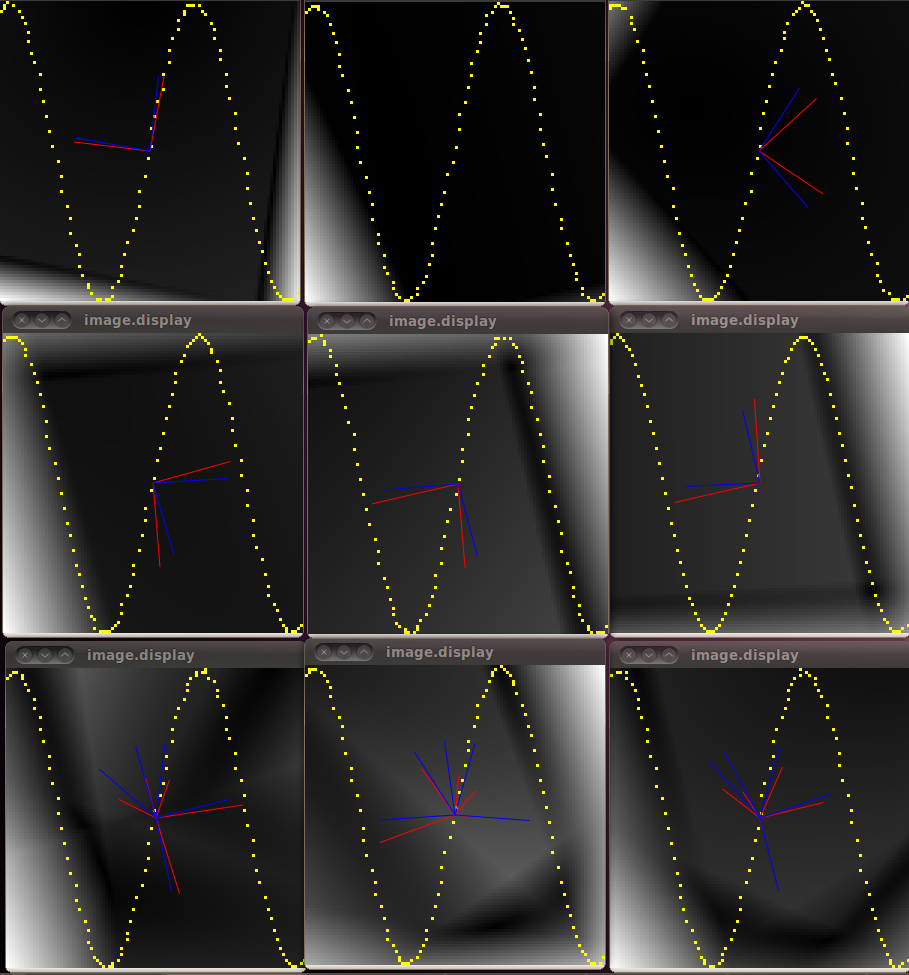
\includegraphics[scale = 0.20]{ramp.png}
\end{center} 
\end{frame} 


\end{document} 